\documentclass[conference]{IEEEtran}
\usepackage{verbatim}
\usepackage{cite}
\usepackage{gensymb}
\usepackage{amsmath,amssymb,amsfonts}
\usepackage{pgf-umlcd}
\usepackage{algorithm}
\usepackage{algpseudocode}
\usepackage{graphicx}
\usepackage{textcomp}
\usepackage{xcolor}
\def\BibTeX{{\rm B\kern-.05em{\sc i\kern-.025em b}\kern-.08em
    T\kern-.1667em\lower.7ex\hbox{E}\kern-.125emX}}
\begin{document}

\title{Algorithms for Two Dimensional Geometry Optimisation\\
{\footnotesize \textsuperscript{}A discussion of alternate approaches for solving the two dimensional geometric optimisation problem using arbitrary bond lengths.}
}

\author{\IEEEauthorblockN{Damon Murdoch}
\IEEEauthorblockA{\textit{School of Information Technology - Computer Science} \\
\textit{Griffith University}\\
Gold Coast, Australia \\
damon.murdoch@griffithuni.edu.au}
}

\maketitle

\begin{abstract}
This is a big yeet
\end{abstract}

\section{Introduction}

Molecular model optimisation is the process of minimising the potential energy of a 
molecule with a given number of atoms, each constrained linearly using unit length bonds.
In the field of computational chemistry, this process is also referred to as geometry 
optimisation. The potential energy of such a system, 'V' is given by the scaled pairwise
addition of Lennard-Jones potentials. The purpose of this investigation is to develop an
algorithm for optimising the geometry of a two dimensional linear bonded molecule of a 
given size 'N' and investigate new, efficient approaches for solving this problem that
take advantage of the features of this problem which separate it from other global
optimisation problems. While this problem operates on an extremely simple representation
of an atom in a two dimensional space, the investigation is useful for developing molecular
structure optimisation algorithms as most algorithms for solving the two dimensional
problem can be translated to higher dimensions without undue complexity.

\section{Literature Review}

A molecule can be defined as "the simplest unit of a chemical substance, usually a group 
of two or more atoms."”(Dictionary,2018). An atom is defined as "the smallest unit of any 
chemical element, consisting of a positive nucleus surrounded by negative electrons."
(Dictionary, 2018). Understanding the stable configurations of a molecule is important 
because it enables us to understand its properties and behaviour with respect to its
structure. When a molecule is constructed using computational chemistry software it may not
be given a stable initial state. This means that if the same molecule were to be constructed
in reaslity, it may be unstable and behave unexpectedly. In order to prevent this, geometry
optimisation is performed to find a stable state for the molecule.

A number of studies have been performed on solving this problem using randomised global search
algorithms such as genetic algorithms or simulated annealing. In some investigations, these
higher-level global search algorithms are accompanied by a local optimisation algorithm, such
as the Limited Memory Broyden Fletcher Goldfarb Shanno algorithm, or L-BFGS. An example of such
a study was published in 1996 by author Wayne Pullan, who developed an in-depth report of numerous
algorithms applied to geometry optimisation for both two and three dimensional problems. 

Based upon previous research, for this investigation it was decided that an interesting and
under explored approach for solving this problem was to optimise each angle individually, one at 
a time in order rather than trying to optimise the entire population at each step. There are several
different approaches using this method which were investigated, and these will be elaborated upon
in the following sections of the report.

\section{Algorithm Description}
\subsection{Section Introduction}

The following section will describe the algorithms which were implemented for testing different
approaches for solving this problem. The algorithms implemented are relatively similar in function
and implementation, and serve the purpose of comparing the efficiency of solving the same problem 
using fundamentally similar methods but approach the order of operations differently.

\subsubsection{Data Structures}

\paragraph{Matrix}

The following data structure is a simplified matrix class which was developed to store the \(r(i,j)\)
components for each molecule object so they could be referred to when calculating the Molecule
system energy rather than recalculating each time the same \(r(i,j)\) is required.\\

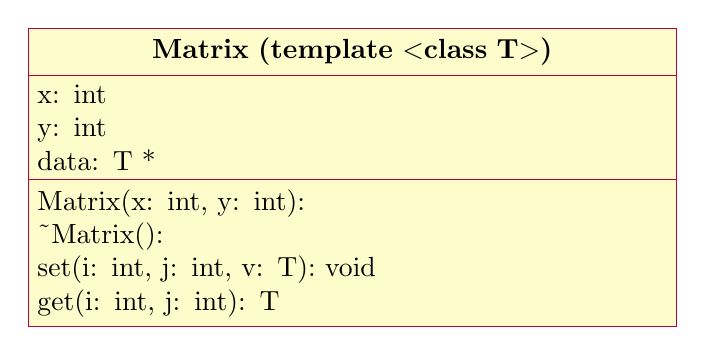
\begin{tikzpicture}
  \begin{class}[text width = 8cm]{Matrix (template $<$class T$>$)}{0,0}
    \attribute{x: int}
	\attribute{y: int}
	\attribute{data: T *}
	
	\operation{Matrix(x: int, y: int):}
	\operation{\~{}Matrix():}
	\operation{set(i: int, j: int, v: T): void}
	\operation{get(i: int, j: int): T}
  \end{class}
\end{tikzpicture}

\paragraph{Point}

The following data structure is a simple point data structure developed for storing the calculated coordinates
for each atom in a Molecule object.\\

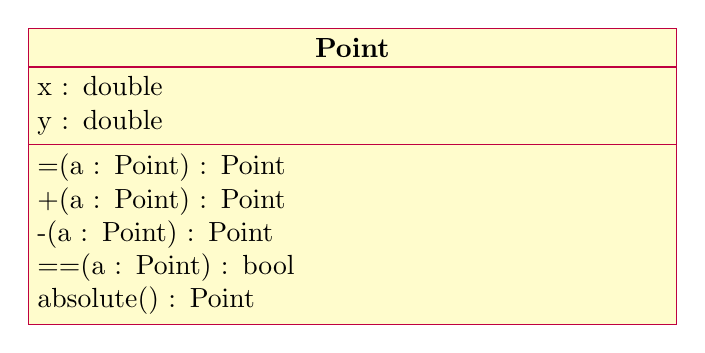
\begin{tikzpicture}
  \begin{class}[text width = 8cm]{Point}{0,0}
    \attribute{x : double}
	\attribute{y : double}
	
	\operation{=(a : Point) : Point}
	\operation{+(a : Point) : Point}
	\operation{-(a : Point) : Point}
	\operation{==(a : Point) : bool}
	\operation{absolute() : Point}
  \end{class}
\end{tikzpicture}

\paragraph{Molecule}

A Molecule class object was implemented for encapsulating all of the data structures necessary for 
defining a molecule with respect to geometry optimisation. a class diagram of the molecule object
is outlined below.\\

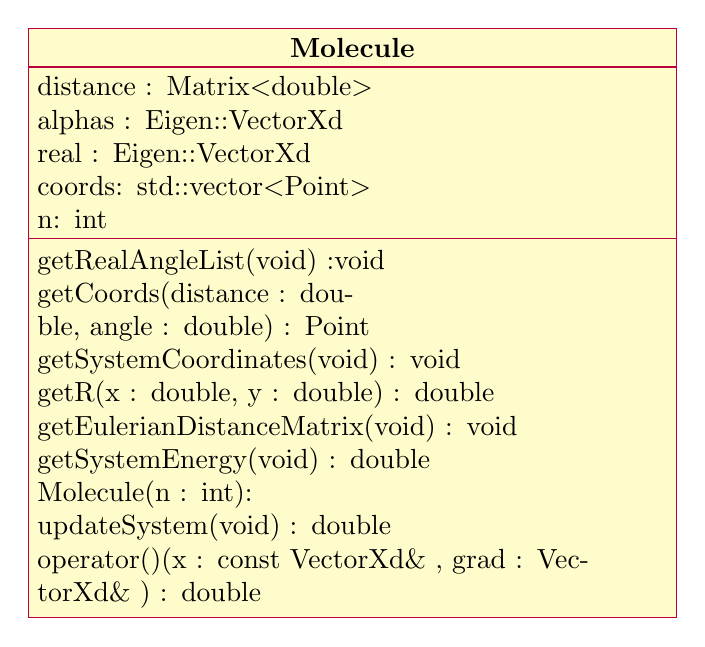
\begin{tikzpicture}
  \begin{class}[text width=8cm]{Molecule}{0,0}
    \attribute{distance : Matrix$<$double$>$}
	\attribute{alphas : Eigen::VectorXd}
	\attribute{real	: Eigen::VectorXd}
	\attribute{coords: std::vector$<$Point$>$}
	\attribute{n: int}
	
	\operation{getRealAngleList(void) :void}
	\operation{getCoords(distance : double, angle : double) : Point}
	\operation{getSystemCoordinates(void) : void}
	\operation{getR(x : double, y : double) : double}
	\operation{getEulerianDistanceMatrix(void) : void}
	\operation{getSystemEnergy(void) : double}
	\operation{Molecule(n : int):}
	\operation{updateSystem(void) : double}
	\operation{operator()(x : const VectorXd\& , grad : VectorXd\& ) : double}
  \end{class}
\end{tikzpicture}

\paragraph{Molecule Function Descriptions}

A number of functions utilised within the Molecule class object are fundamental to the operation of the 
overarching algorithms, and their function will be demonstrated in this section.

%\begin{comment}

\begin{algorithm}
  %\Procecure{Molecule::getRealAngleList()}{$x$}
  
  %\EndProcedure
\end{algorithm}

\begin{algorithm}
  %\Procecure{Molecule::getSystemCoordinates()}{$x$}
  
  %\EndProcedure
\end{algorithm}

\begin{algorithm}
  %\Procecure{Molecule::getEulerianDistanceMatrix()}{$x$}
  
  %\EndProcedure
\end{algorithm}

\begin{algorithm}
  %\Procecure{Molecule::getSystemEnergy()}{$x$}
  
  %\EndProcedure
\end{algorithm}

\begin{algorithm}
  %\Procecure{Molecule::updateSystem()}{$x$}
  
  %\EndProcedure
\end{algorithm}

\begin{algorithm}
  %\Procecure{Molecule::operator()}{$x$}
  
  %\EndProcedure
\end{algorithm}

%\end{comment}

\subsection{Ordered Single Pass $\alpha$ Optimisation}
\subsubsection{Discussion}

This algorithm follows the application of an extremely strict annealing algorithm, which randomly
optimises $\alpha_m$ in order $\alpha_0$ ... $\alpha_{n-1}$. This search is performed by iteratively
assigning each $\alpha$ a value in the range of {-180$\degree$...180$\degree$} until a maximum number of
iterations have been performed. Once the maximum is reached the algorithm performs the same steps on the 
next $\alpha$ variable.

\subsubsection{Pseudocode}


\subsection{Standard Annealing $\alpha$ Optimisation}
\subsubsection{Discussion}
\subsubsection{Pseudocode}


\subsection{Brute Force $\alpha$ Optimisation}
\subsubsection{Discussion}
\subsubsection{Pseudocode}



\begin{thebibliography}{00}
\bibitem{b1} Dictionary, a. (2018). atom Meaning in the Cambridge English Dictionary. [online] 
Dictionary.cambridge.org.
Available at: https://dictionary.cambridge.org/dictionary/english/atom [Accessed 24 Jul. 2018]
\bibitem{b2} Dictionary, m. (2018). molecule Meaning in the Cambridge English Dictionary. [online] Dictionary.cambridge.org.
Available at: https://dictionary.cambridge.org/dictionary/english/molecule [Accessed 24 Jul. 2018]
\bibitem{b3} shodor.org. (2018). Background Reading for Geometry Optimizations. [online]
Available at: https://www.shodor.org/chemviz/optimization/students/background.html [Accessed 24 Jul. 2018]
\bibitem{b4} Structure.usc.edu. (2018). Minimization and Molecular Dynamics. [online]
Available at: http://structure.usc.edu/mmtk/MMTK 4.html [Accessed 24 Jul. 2018]
\bibitem{b5} Jean, M. (2018). Energy Minimization Methods. [online] About.illinoisstate.edu.
Available at: https://about.illinoisstate.edu/standard/Documents/CHE%20380.37/Handouts/380.37emin.pdf [Accessed
25 Jul. 2018].
\bibitem{b6} Clark, S. (2018). Geometry Optimization. [online] Cmt.dur.ac.uk.
Available at: http://cmt.dur.ac.uk/sjc/thesis dlc/node37.html [Accessed 26 Jul. 2018].
\bibitem{b7} Ul-Haq, Z. (2018). Introduction to Geometry Optimization. [online] Th.fhi-berlin.mpg.de.
Available at: https://th.fhi-berlin.mpg.de/sitesub/meetings/dft-workshop-2016/uploads/Meeting/May 6 Qasmi.pdf
[Accessed 26 Jul. 2018].
\bibitem{b8}Spindynamics.org. (2018). molecular geometry optimization. [online]
Available at: http://spindynamics.org/documents/cqc lecture 6.pdf [Accessed 26 Jul. 2018]
\bibitem{b9}Helgaker, T. (2009). Geometry optimization. [online] Folk.uio.no.
Available at: http://folk.uio.no/helgaker/talks/ESQC09 Optimization.pdf [Accessed 26 Jul. 2018]
\bibitem{b10}Openmopac.net. (2018). The BFGS function optimizer. [online]
Available at: http://openmopac.net/manual/BFGS optimizer.html [Accessed 26 Jul. 2018].
\bibitem{b11}Tcm.phy.cam.ac.uk. (2018). CASTEP Geometry optimization. [online]
Available at: https://tinyurl.com/thcastepgeomopt
[Accessed 26 Jul. 2018].
\bibitem{b12}Cpmd.org. (2018). Geometry Optimization. [online]
Available at: http://www.cpmd.org:81/manual/node80.html [Accessed 26 Jul. 2018].
\bibitem{b13}General methods for geometry and wave function optimization Thomas H. Fischer and Jan Almlof
The Journal of Physical Chemistry 1992 96 (24), 9768-9774 DOI: 10.1021/j100203a036
\bibitem{b14}Tcm.phy.cam.ac.uk. (2018). CASTEP. [online]
Available at: https://preview.tinyurl.com/abtcastep [Accessed 26 Jul. 2018].
\bibitem{b15}Clark, S. J.; Segall, M. D.; Pickard, C. J.; Hasnip, P. J.; Probert, M. J.; Refson, K.; Payne, M. C.
”First principles methods using CASTEP”, Zeitschrift fuer Kristallographie, 220 (5-6), 567-570 (2005
\bibitem{b16}Pullan, WJ 1996, Global optimisation applied to molecular architecture, 
PhD thesis, Central Queensland University, Rockhampton. http://hdl.cqu.edu.au/10018/26734
\end{thebibliography}

\end{document}